\documentclass[10pt, preprint, nonatbib]{sigplanconf}
\usepackage{times,epsfig,endnotes,graphicx, verbatim}
\usepackage{datetime, url, pdfpages}

\conferenceinfo{SOSP'17}{October 29--31, 2017, Shanghai, China}
\copyrightyear{2017} 


% These only appear when the 'preprint' option is specified.
% Enabling these will cause the first page of the document to fail the 
% format check on HotCRP :-(
%\titlebanner{Under submission to SOSP 2017 - do not cite or distribute}
%\preprintfooter{Draft of {\currenttime}, \today{}}

% No date in title area.
\date{}

% Paper number and no. of pages as author
\authorinfo{Paper \textbf{\#224}}{NN pages}


\begin{document}

%make title bold and 14 pt font (Latex default is non-bold, 16 pt)
\title{\Large \bf Cyclone: Warp Speed Replication for Key Value Stores}

\maketitle

% Use the following at camera-ready time to suppress page numbers.
% Comment it out when you first submit the paper for review.
%\thispagestyle{empty}

\begin{abstract}
Persistent key value stores are rapidly becoming an important component of many
distributed data serving solutions - with innovations targeted at taking
advantage of growing flash speeds. Unfortunately their performance is hampered
by the need to maintain and replicate a write ahead log to guarantee
availability in the face of machine and storage failures. Cyclone offers a
solution to this problem by leveraging a small amount of directly attached
non-volatile memory (NVM) such as NVDIMMs to maintain a two level log - the upper
level in a small amount of NVM draining into a larger lower level log
maintained on flash. Replicating the smaller log kept in NVMs transforms the
replication problem into a packet switching problem - the leader sends the exact
same packet to all follower replicas and we solve the problem as such by using
the RAFT protocol implemented as a software multicast module on the Data Plane
Development Kit (DPDK). Second, we levergage the observation that key value store
interfaces are commutative for operations to different keys to scale our two
level log horizontally into a number of physical two level logs - with a hash of
the key being used to choose the right log. Each log is replicated by an
independent instance of RAFT, thereby leveraging the scalability afforded by
classic software packet switching when using multiple CPU cores. Cyclone is able
to replicate millions of small updates a second using only commodity 10 gigabit
ethernet adapters and improves the performance of RocksDB - a popular persistent
key value store by orders of magnitude when compared to its own write ahead log
without replication.
\end{abstract}

\section{Introduction}

\section{Two Level Log}
A fundamental challenge in building an efficient replicated log is dealing with
network overheads. Cyclone'e construction is predicated on the observation that
in the common case protocols such as RAFT simply multicast the same entry
received from a client, from the leader replica to all follower replicas. This
suggests that an efficient way to implement a replicated log is to treat it as a
software packet switching problem. However peristing logs on flash represents an
impediment in that block storage devices are not good candidates to hold packets
being software switched. Our solution is to split the log into two levels. The
upper level is held in persistent directly attached non-volatile memory (NVM)
such as NVDIMMs. The lower level is held on a flash SSD - we term the lower
level log as the flash log. We periodically drain entries in batches from the
NVM log to the backing flashlog. An important and beneficial side effect of this
two level approach is that we need only limited amounts of NVM with the bulk of
the log residing on flash - an arrangement that maps well to the relative cost
of the two types of memory. We begin by describing the NVM log and how we
implement the RAFT consensus protocol in the packet switching paradigm around
it. We then describe the flashlog and how we drain entries in batches from the
NVM level to the flash level.

\subsection{NVM Log}
The NVM log is maintained as a circular log of fixed sized pointers (a pointer
log) to memory buffers - each of which holds a client request. This arrangement
is shown in Figure~\ref{fig:nvm_log} that also illustrates the advantage of
such an arragement. Adding a level of indirection in the NVM log allows us to
isolate the circular log being manipulated by the RAFT protocol from the
problems of variable sized client requests that can be scattered across
non-volatile memory depending on the internals of the memory allocator of the
packets switching library we use. Another advantage is that it makes recovery
from NVM easy - appends to the circular pointer log are atomic and we use the
pointer log to recover allocator state i.e. what pieces of NVM are currently in
use by the log.

\begin{figure}
\centering
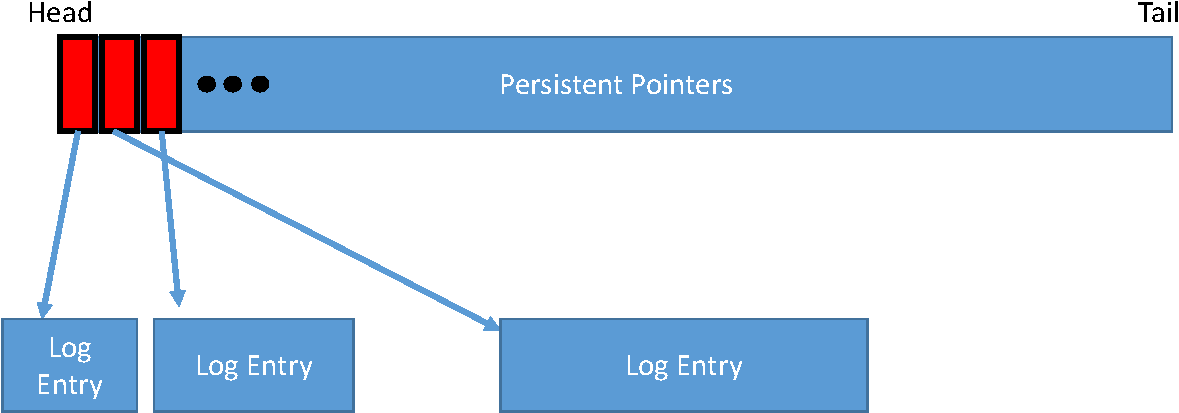
\includegraphics[scale=0.3]{figures2/nvm_log.pdf}
\caption{NVM Log Structure}
\label{fig:nvm_log}
\end{figure}

We now describe how we implement the RAFT consensus protocol to replicate the
NVM log across a set of replicas. The software packet switching idea we apply is
to separate the control plane from the dataplane using the Data Plane
Development Kit (DPDK~\cite{dpdk}) library for direct userspace access to the
network interface.

\subsubsection{Dataplane Separation}
We use RAFT~\cite{raft} as the underlying protocol for log replication. RAFT
replicates a log across a set of replicas. Its operations are leader-based and
RAFT incorporates a leader election algorithm that elects a leader with the most
upto date log. The leader receives log entries from clients, appends them to the
persistent log (NVM log in this case) and multicasts the new entry to follower
replicas. On a response from enough follower replicas (constituting a majority
quorum) the leader replica can then execute the command in the log entry. In
our case this involves accessing the key value store and sending the response
back to the client.

We implement the common case flow in RAFT as a software packet switch using
DPDK. The dataplane now encompasses the NIC and the CPU caches with the NIC
placing packet data directly in the CPU cache via DDIO~\cite{ddio} - a standard
feature of most NICs today. The dataplane for the RAFT protocol is therefore
separated from the control plane. The control plane now runs on a CPU core and
takes care of checking adherence to the protocol: checking for correct term, log
index and that the replica receiving the packet from the client is indeed the
leader. In addition, the control plane is responsible for non common-case
activities such as dealing with timeout and leader elections.

The pseudocode in Figure~\ref{fig:control_plane} describes the control plane in
Cyclone organized as event handlers triggered on receiving a packet. We focus on
two events for illustration (and brevity): the event where a request is received
from a client and the event where a leader election related message is
received. A key concern when we built Cyclone was adhering as far as possible to
the software packet switching principle of separating the control plane from the
dataplane. This means that the CPU should avoid examining every byte of the
packet as far as possible.

If an election message is received all the code related to handling
the election related message is run on the CPU core and all contents of the
packet are examined to decide what to do in accordance with the RAFT protocol
state machine. This is an exception to the software packet switching principle
but one that we found acceptable since leader elections are rare compared to the
common case of replicating client packets.

The sequence of operations when a packet is received from the client however
needs careful design for efficient software packet switching. To illustrate how
this is achieved, Figure~\ref{fig:packet_layout} shows how Cyclone manipulates
packet layouts across the two steps of prepending a RAFT header and transmitting
to follower replicas. DPDK describes packets using an ``mbuf'' data
structure. Roughly speaking, an ``mbuf'' consists of a flat array of bytes
actually containing the byte and a fixed size piece of external metadata that
describes various aspects of the packet, most crucially a pointer to the start
and end of the packet in the byte array. DPDK's userspace drivers receive
packets from the NIC such that they are offset in the byte array by a
configurable amount referred to as ``headroom''. We strip off the existing
network headers in the packet and prepend RAFT related information specific to
each log entry in the headroom by shifting the start pointer appropriately -
these operations are standard enough for software packet switches that DPDK
provides convenient library calls to do it. For the final step, we need to
prepare the packet for transmission to the various follower replicas. To do this
we prepare a different packet containing an ethernet header for the targeted
replica and ``chain'' the data packet to each of these headers. Each header is
then separately handed off to the driver for transmission via the NIC, carrying
the data packet with it by association.

\begin{figure}
\begin{verbatim}
    event_receive_client_req()
    {
      if(!check_is_leader()) {
        drop_msg
        return
      }
      Prepend raft log term and index
      Persist to local log
      Transmit to follower replicas
    }

    event_receive_election_msg()
    {
      Handle_election_msg()
    }
\end{verbatim}
\caption{Cyclone Control Plane Fragment}
\label{fig:control_plane}
\end{figure}

\begin{figure}
  \centering
  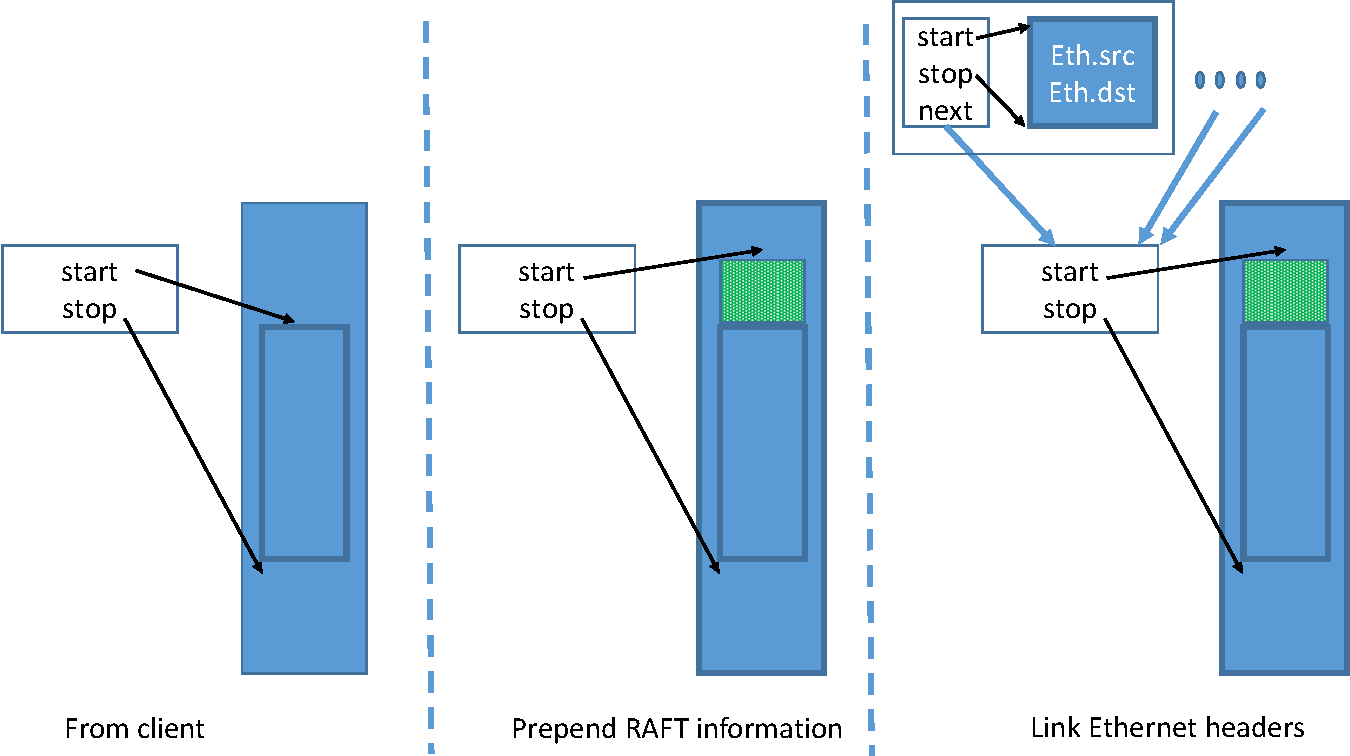
\includegraphics[scale=0.3]{figures2/network_packet.pdf}
  \caption{Cyclone Network Packet Layout}
  \label{fig:packet_layout}
\end{figure}

We note that by discrding stream oriented protocols the network layer is not
longer reliable or ordered. This is not a problem for RAFT that is designed to
tolerate network failures resulting in drops or reordering of network
packets. However this rules out consensus protocols such as Zookeeper Atomic
Broadcast (ZAB~\cite{zab}) that depend on a reliable stream-oriented network
layer to function correctly.

Finally, we turn our attention to the persistence step in
Figure~\ref{fig:control_plane}. RAFT requires that the log entry be persisted
before it is multicast out to follower replicas. Since the NVM is directly
attached we do this by executing a cacheline flush ({\tt clflush}) instruction
for every cacheline in the packet and the pointer in the pointer buffer to
persist these via the memory bus. This is the one exception to our otherwise
clean separation between the control and data plane - necessitated by the fact
that at the moment NICs do not support persistent memory. This is not too
onerous a burden because we can use the newly introduced {\tt
  clflush-opt}~\cite{clflush_opt} instruction specifically intended to
efficiently flush to persistent memory without the overhead of the serialization
normally introduced by {\tt clflush}. This allows one to hit full memory
bandwidth on present generation platforms, a quantity in excess of 200 Gb/s per
core, well above the near term speeds of network interface cards.

\begin{figure}
  \centering
  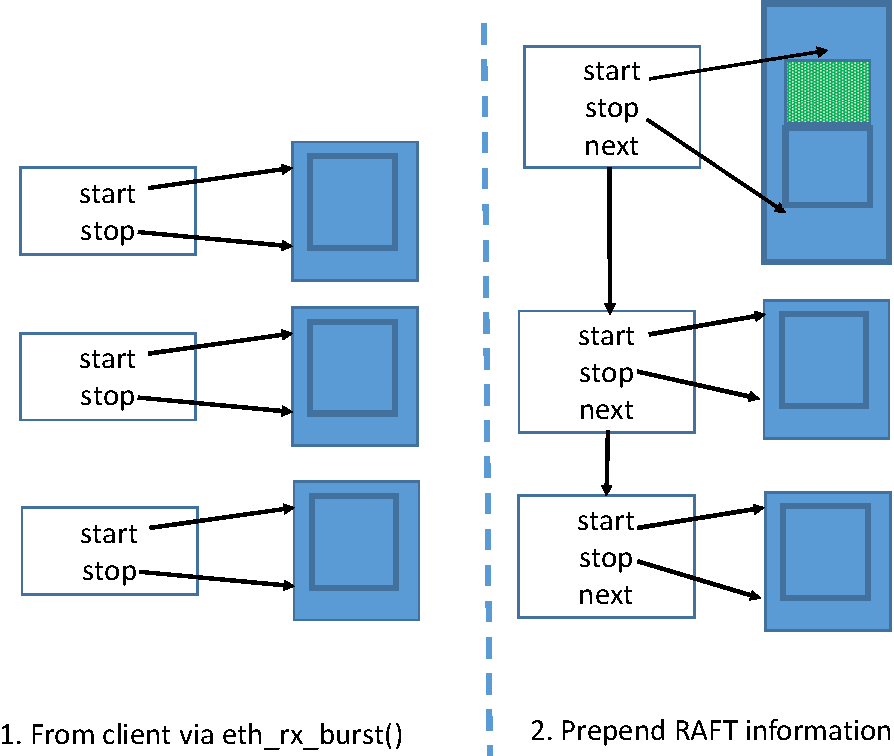
\includegraphics[scale=0.3]{figures2/batching.pdf}
  \caption{Batching}
  \label{fig:batching}
\end{figure}

\subsubsection{Batching}
Although the control plane code only runs operations related to the RAFT state
machine it is still slow enough relative to the dataplane to add significant
overhead for each packet. We tackle this problem by applying another classic
software packet switching technique: batching - illustrated in
Figure~\ref{fig:batching}. We use a burst receive call available in the DPDK
userspace driver to receive a burst of client packets at a time. We then chain
these packets together and treat them as a single log entry from the perspective
of RAFT, amortizing the control plane overheads over the packets (at most 32 at
a time due to current driver limitations).

We note there that batching in Cyclone does not involve a latency-throughput
tradeoff like in many other systems~\cite{ix-dataplane}. The batch receive call
we use in DPDK returns immediately with whatever number of packets is available,
including zero. We always flush the transmit buffer after every call to DPDK to
transmit packets to replicas. Therefore, we never tradeoff latency for
throughput when batching. 

\subsection{Flash Log}
Cyclone is designed to use only limited amounts of NVM and drains log entries
down into a log placed on a flash SSD - that we term the flashlog. The flashlog
is written out in segments of configurable size (we use 128KB segments). A
segment buffer is prepared in memory (volatile DRAM) using the layout shown in
Figure~\ref{fig:flashlog_page}. We do not allow objects in the flashlog to cross
a 4KB boundary - linking multiple objects together with a special flag encoded
into the size if necessary. We flush log segments out to the log file using
asynchronous direct IO, and therefore we fill one log segment buffer while
keeping IO to another one outstanding to the flash drive. To avoid having to do
a synchronous metadata flush, we preallocate (using the posix\_fallocate call) a
gigabyte worth of zero filled disk pages at the end of a file, at a time.

In order to recover from a crash, we make two important assumptions about the
underlying SSD. First, we assume that 4KB is the \emph{minimum} atomic unit for
updating pages on the SSD even under power failure i.e. there are no shorn
writes on a 4KB page~\cite{shorn_writes}. We also assume that the SSD has power
loss data protection meaning that writes cached in the drive's volatile cache
are written to the SSD using a backup capacitor in the event of power failure -
a property of many data center class SSDs today, including the Intel DC P3600
SSD~\cite{ssd_spec} we use in our evaluation. Together these two assumptions
mean that we can recover a consistent prefix of the log on a power failure.

We move log entries from the head of the NVM log to the flashlog buffers in FIFO
order. THe NVM log entry is only actually removed then the IO for the
corresponding flashlog page is complete. This means that during recovery we can
have the same log entry both in the NVM log and the flashlog, a condition that
can be detected by examining the RAFT related information that is embedded as
part of the logged packet.


\begin{figure}
  \centering
  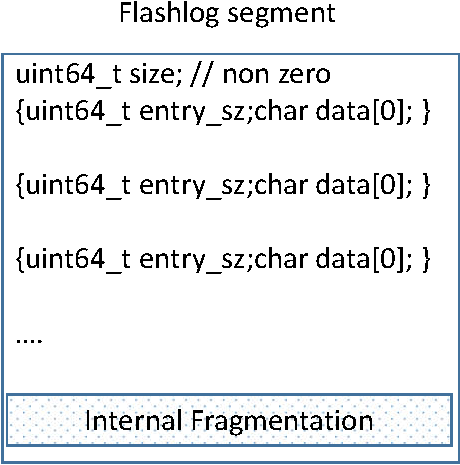
\includegraphics[scale=0.3]{figures2/flashlog_page.pdf}
  \caption{Flashlog segment}
  \label{fig:flashlog_page}
\end{figure}

The fact that we can immedately absorb updates into an NVM log and only move
them to the flashlog in suitable units for block IO, sidesteps a common problem
with logging to secondary storage - the need to do group commit. Logging systems
often wait to collect a batch of entries to write to secondary storage trading
latency for throughput. This is unnecessary in Cyclone as it effectively makes
use of directly attached NVM with a two level log that removes the need to make
this tradeoff.

\begin{figure}
  \centering
  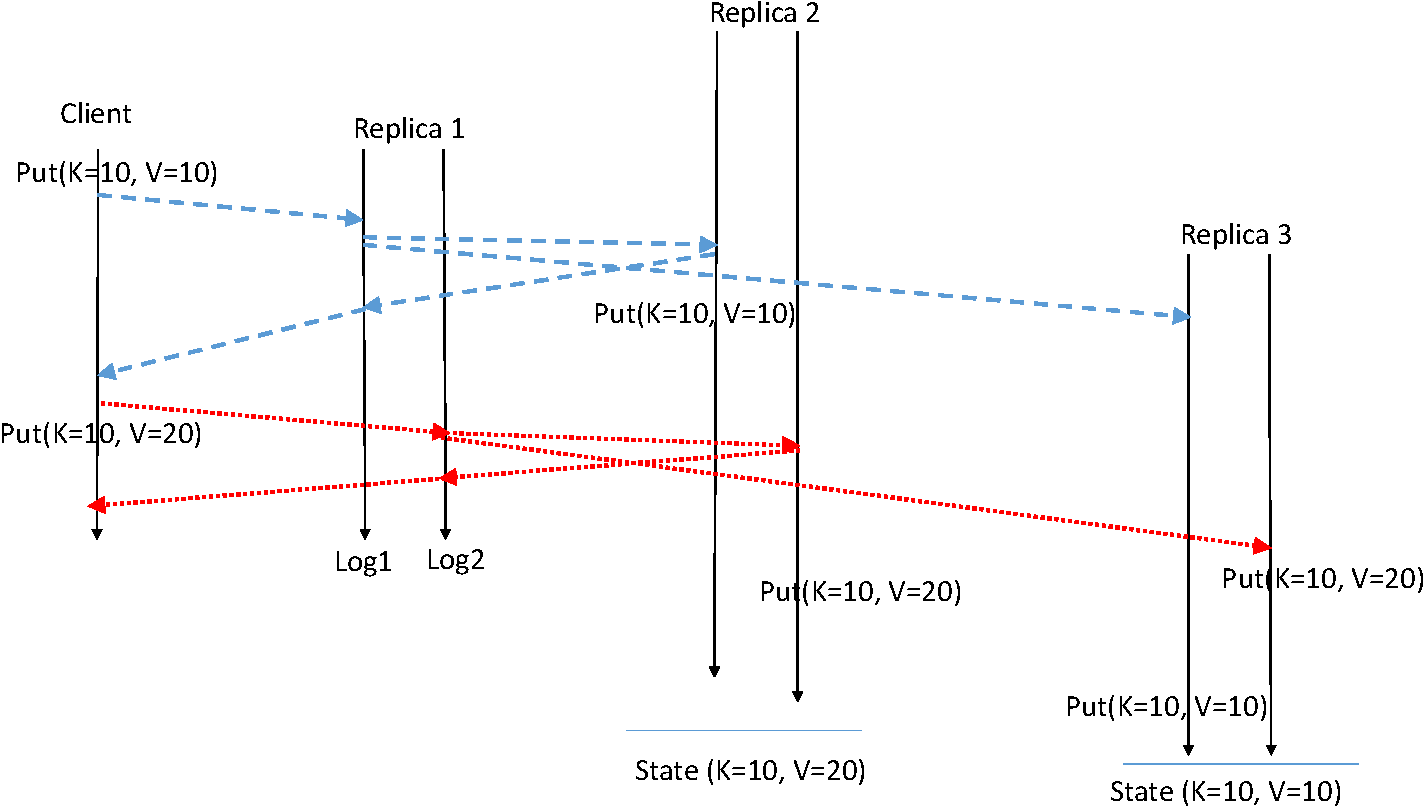
\includegraphics[scale=0.3]{figures2/race.pdf}
  \caption{Race with multiple physical logs}
  \label{fig:race}
\end{figure}

\section{Horizontal Scaling}
The basic principle in Cyclone is to turn log replication into a software packet
switching problem. A key ingredient in software packet switching is applying
multiple CPU cores to parallelize the control plane, scaling message processing
throughput. In this section we describe how we can horizontally scale Cyclone's
single \emph{logical} log across multiple \emph{physical} logs. For each
physical log, we run an independent version of RAFT with the corresponding
control plane mapped to a dedicated core. Further, as we shortly describe we
assume a concurrent key value store where a set of CPU cores independently run
operations from the physical logs on the shared memory key-value store data
structure, synchronizing as necessary.

We begin by describing how a key-value store API can be mapped on these
independent physical logs without divergence in replica state. We then discuss
how different pieces of work related to replication and the key value store
itself are distributed across available CPU cores and available NIC queues. 

\subsection{Leveraging API Commutativity}
Update requests to a key-value store consist of a key and an associated operation -
such as ``put'' that set the value for the key or ``merge'' that calls a
user-defined operator to merge a new value for the key into the existing value.
A naive approach that maps a key to a random physical log and subsequently to a
random core on the system for execution runs into the determinism problem -
replicas could diverge with respect to the final value assigned to a key on
different replicas. We illustrate this problem with an example in
Figure~\ref{fig:race} where two updates to the same key race with each other on
different physical logs and execution cores to end up being applied in different
orders on different replicas, leading to a divergence of state.

The solution to this problem is observe that the key-value store is a concurrent
data structure that ultimately admits a serialization of operations to
it. Further, consecutive operations to different keys in the serial history can
be interchanged, because operations to different keys are
\emph{commutative}. The correct way to use different physical logs is therefore
to simply hash the key to select the physical log \emph{and} the core on which
the operation executes. This guarantees determinism as the serial history of
two different replicas can be transformed into the same serial history by
reordering operations to different keys. 

Further relaxations to the mapping scheme are possible when operations to the
same key are also commutative. A good example is when key value stores are used
to maintain counters. Different increment operations to the same counter are
commutative if one is prepared to tolerate non-determinism in the sequence of
updates seen by a reader with the counter reaching the same eventual value. This
specific use-case, in fact, lead to the addition of the merge operation in
Rocksdb, a key value store that we use for evaluation. Merge operations
therefore could be dispatched to a random physical log with no harm. For this
paper however, we stick on the stricter requirement that operations to the same
key are not commutative.

\subsection{Core Assignment}

TBD: mention no linearizability for reads at the moment

\subsection{NIC Queue Assignmnt}

\subsection{Ganged Operations}

\section{Evaluation}
We evaluate Cyclone on a 12 node cluster connected via a 10 GigE switch. Three
of the machines are equipped with 1.6TB Intel DC P3600 SSDs and 4*10 GigE
ports. The remaining nine machines do not have SSDs and have only one 10 GigE
port, serving as clients for most of the experiments. As with other
work~\cite{faast}, we use DRAM on the machines to proxy for NVDIMMs where
necessary - the persistent memory needed never exceeds 64 MB regardless of the
size of the key value store or second level log on flash. We divide the
evaluation into three parts. First, we evaluate Cyclone's performance with a
single level log as a pure software packet switch. Next, we evaluate performance
when adding a second level of log on flash. Finally, we evaluate performance
when integrated with Rocksdb as an alternative to Rocksdb's write ahead
log. Unless otherwise mentioned, we use a 60 byte header followed by a payload
for experiments. We log both the header and payload. In all cases the server
echoes the received entry (header and payload) back to the client. We fix the
number of application threads at 32 using at most 8 threads for running RAFT
instances.

Cyclone is built on top of DPDK to apply software packet switching techniques to
the log replication problem. We therefore begin by systematically evaluating
optimizations applied in Cyclone to replicate the top level log in
Figure~\ref{fig:network_opts} - with no payload. The y-axis reports latency seen
at the client (which means two network round trips with replication). Using
TCP/IP to replicate a RAFT log tops out at around 30K entries/s. Applying
optimizations improves performance by a large enough amount that we use a log
scale on the x-axis. Switching to DPDK (the line marked +DPDK) improves the
throughput by an order of magnitude to around 50K entries/s. Using batching
(line marked +batching) improves the performance further bringing us close to a
million entries/s. Scaling horizontally to 8 physical logs (+8 phy logs)
improves performance to close to 2M entries/s. Finally using all 4 ports on the
machine to replicate entries improves performance considerably to 6M
entries/s. In all performance improves by 200X over the TCP/IP single log
baseline. Cyclone also considerably improves the latency for replication, from
close to 100us with TCP/IP to around 30us at peak throughput.

\begin{figure}
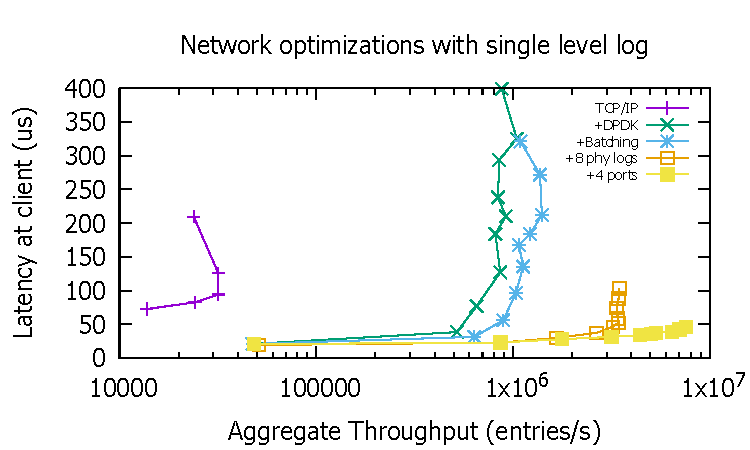
\includegraphics[scale=0.6]{results2/network_opts.pdf}
\caption{Network optimizations for top level log}
\label{fig:network_opts}
\end{figure}

There are two factors that can have significant impact on Cyclone's
performance. First, the number of replicas dictates the outgoing message rate
from the leader replica and therefore increasing the replication factor can
decrease Cyclone's performance. Figure~\ref{fig:replicas} shows the impact of
varying replica count. Using only a single replica cuts out a network round trip
and shows the best unloaded latency (10 us) and peak throughput (near 10M
entries/s). Adding replicas decreases the peak throughput down to around 2M
entries/s. We note that a number of previous pieces of work~\cite{faast, farm}
use three replicas and therefore we focus on three replicas for the replicated
cases we consider below. The second factor that dictates Cyclone's performance
is the size of the log entry being replicated. Figure~\ref{fig:payload} shows
the effect of increasing the payload size from zero to 512 bytes. Peak
throughput drops from 6M entries/s to approximately 2M entries/s. At this
replication rate, the leader replica needs to transmit data at approximately 30
Gbit/s. Coupled with the cost of network headers all four 10 GigE ports are now
saturated and therefore Cyclone hits the network line rate bottleneck at this
point.

\begin{figure}
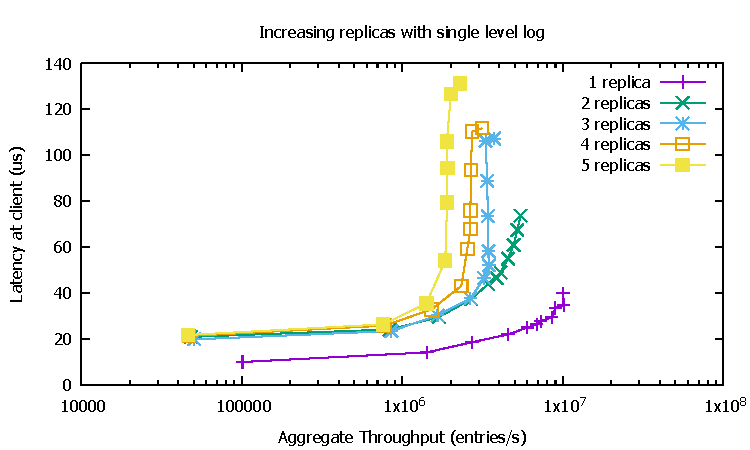
\includegraphics[scale=0.6]{results2/replicas.pdf}
\caption{Impact of replica count}
\label{fig:replicas}
\end{figure}

\begin{figure}
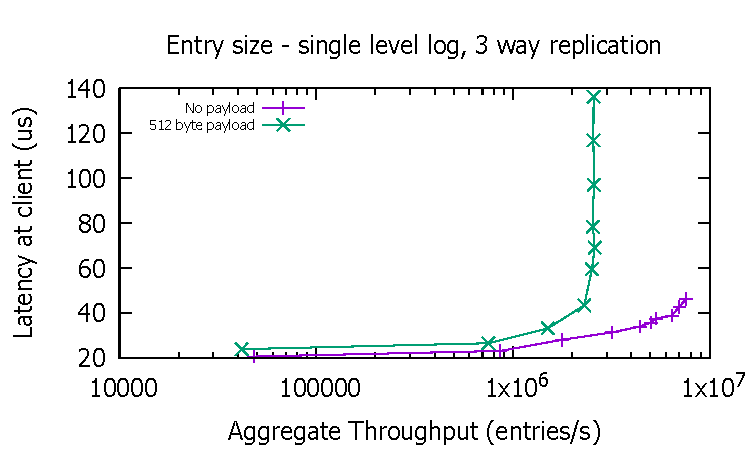
\includegraphics[scale=0.6]{results2/512.pdf}
\caption{Impact of payload size}
\label{fig:payload}
\end{figure}

We now turn our attention from the network component of Cyclone to the storage
one by adding the second level flashlog. We evaluate the impact of adding
storage to our hitherto pure packet switching scenario in
Figure~\ref{fig:flashlog}. Batching entries from the top level NVDIMM log to the
second level flashlog is clearly beneficial as adding flash storage at the
second level has almost no impact on peak performance in Cyclone for small
entries. The situation however changes for larger
entries. Figure~\ref{fig:flashlog_512} shows that using a 512 byte payload has a
significant impact on peak throughput - it drops to approximately 350K
ops/sec. This corresponds to around 50K 4KB IOPS to the SSD to write out the
flashlog pages. The peak for the drive is 160K IOPS using a queue depth
(concurrency) of 128. With 32 application threads we expect a lower peak
throughput around 40K IOPS explaining our bottleneck at 50K IOPS.  It is
possible to tune our observed performance further by aligning the flush boundary
to increase the number of outstanding requests - we do not do so in this paper,
keeping Cyclone agnostic to the exact size of entry being replicated. A final
point about Figure~\ref{fig:flashlog_512} is that once we are past the storage
bottleneck the latency spike is dramatic and large enough to trigger Cyclone's
failure detector and repeated retries from the clients. There are - therefore -
no points on the ``knee'' of the curve as in the pure packet switched one level
log case.

\begin{figure}
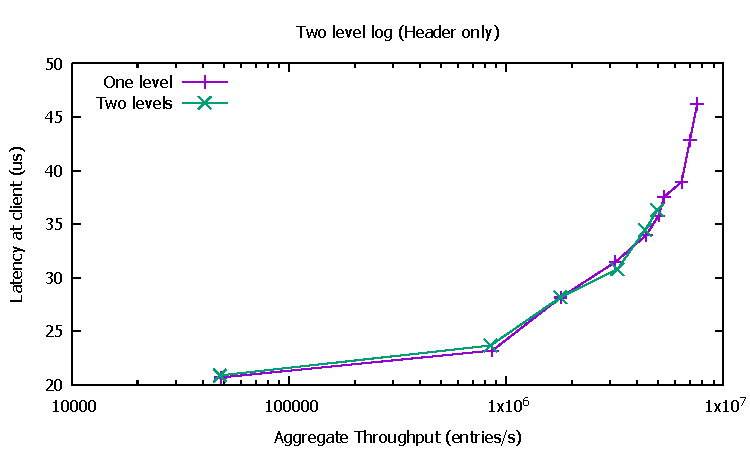
\includegraphics[scale=0.6]{results2/flashlog.pdf}
\caption{Impact of adding second level log}
\label{fig:flashlog}
\end{figure}

\begin{figure}
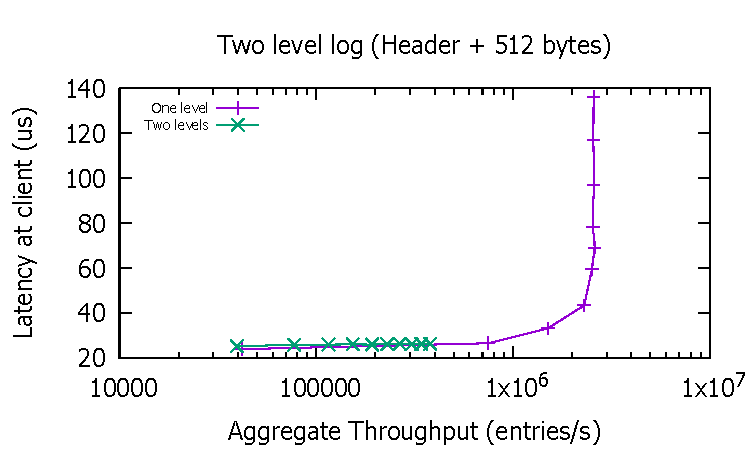
\includegraphics[scale=0.6]{results2/flashlog_512.pdf}
\caption{Impact of adding second level log (512 bytes payload)}
\label{fig:flashlog_512}
\end{figure}

The final dimension we evaluate is of ganged operations. The primary purpose of
ganged operations is to avoid the need for distributed transactions to
manipulate what is a single shared memory image and therefore we were most
concerned about unloaded latency given the complexity of synchronizing different
replication quorums as well executing our rendezvous protocol on multiple
cores. We therefore setup an experiment where a single client reflecting the
unloaded case made ganged requests to the replicas. We varied the number of
cores participating in the request from one to the full complement of 32
application cores. Figure~\ref{fig:ganged} shows the results both using a single
level log as well as a two level log. The primary takeaway is that unloaded
latency increases slowly as we increase the number of active cores - to around
40 us from the baseline of 20 us. There are two causes of this. First, there is
a rapid increase from 1 to 8 active cores, the reason being that this
corresponds to an increase in the number of quorums that must be synchronized
on. There is some amount of synchronization involved in the userspace DPDK
driver for access to common resources for accessing the NIC and this affects the
ability to simultaneously issues replication messages on all quorums. The
smaller contribution to increasing latency that continues past the 8 core case
is due to cacheline pingponging when executing the rendevous. Both these sources
of latency drift could be corrected using replication quorums mapped to
dedicated NICs and more scalable rendezvous designs (such as with machine aware
broadcast trees~\cite{broadcast_tree}). However we deemed the complexity of such
optimizations unnecessary. The added latency for most cases is well under the
extra round trip delay, which would the minimum needed for a solution using
distributed transactions via two phase commit.

\begin{figure}
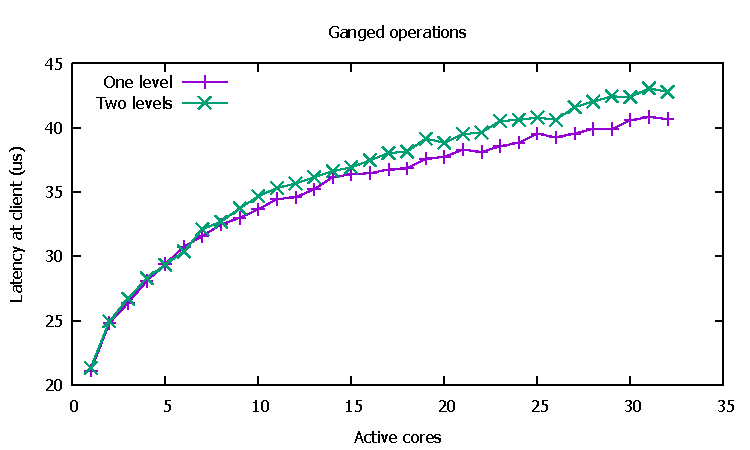
\includegraphics[scale=0.6]{results2/multi.pdf}
\caption{Ganged Operations}
\label{fig:ganged}
\end{figure}

We now evaluate Cyclone integrated with the Rocksdb persistent key value
store. Rocksdb is a complex industrial strength persistent key value store and
this means that it is accompanied by a complex array of performance tuning knobs
to get the best performance from flash. We were also aware that SSD performance
is slated for dramatic increases in the coming years with the introduction of
new memory technology such as 3DXPoint based Optane SSDs. To demonstrate that
Cyclone is future proof we eliminated flash media performance from the picture
as far as the key value store is concerned by placing all files for the key
value store (SSTables) on a RAMdisk, which presumably represents the limit in
performance for flash in the near future. All log files on secondary storage
however - both Rocksdb's own write ahead log and the alternative of Cyclone's
second level flashlog - are placed on the SSDs.

We evaluate two different request sizes: 8 byte keys with 8 byte values and 8
bytes keys with 256 byte values. We run 8 physical logs on 8 cores and devote 32
cores to making requests to Rocksdb. Since we are interested in performance of
the log, which is only used for update requests, our workload is 100\% writes.

Before evaluating with Rocksdb we measure the baseline performance of
replicating the log with Cycloine for the given request sizes - Rocksdb performs
a no-op. We note that in addition to the key and value, we are also logging
RocksDB specific request data such as operation type and the request header.
Figure~\ref{fig:kv_baseline} shows the baseline performance for the chosen
request sizes. With the smaller request size, Cyclone can conservatively sustain
close to a million requests a second at a latency of just under 25us. With the
larger request size, Cyclone can sustain around 350K requests a second, again at
a latency of just under 25 us. Armed with these baseline numbers we now examine
how well Cyclone performs with Rocksdb.

\begin{figure}
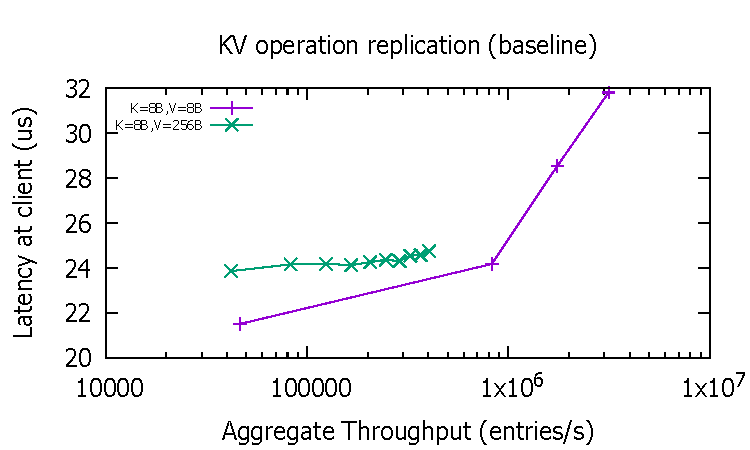
\includegraphics[scale=0.6]{results2/kv_baseline.pdf}
\caption{Baseline KV replication performance}
\label{fig:kv_baseline}
\end{figure}

The performance of Rocksdb with Cyclone for the small update workload is shown
in Figure~\ref{fig:rocksdb}. We consider four different settings. The line
labeled Rocksdb is the key value store running with no logging whatsover - a
system crash would lead to data loss. The line labeled Rocksdb/WAL is for
Rocksdb running with its write ahead logging turned on. The large gap between
these two is the overhead of the existing Rocksdb WAL solution. The line labeled
Rocksdb/Cyclone 1 way is a two level Cyclone log but without any
replication. The line almost exactly tracks the performance of Rockdb. As
suggested by the baseline replication performance, Cyclone is able to provide a
write ahead log with no overhead to Rocksdb. The line labeled Rocksdb/Cyclone 3
way is with 3-way replication turned on. Other than a 20us delta due to the
extra network round trip, the line almost exactly tracks the Rocksdb no logging
case. Cyclone therefore provides high availability to Rocksdb at a fraction of
the cost of its existing single machine write ahead log. We also repeat the
experiment for the larger update size in Figure~\ref{fig:rocksdb_256}. The
conclusions are identical: Cyclone solves Rocksdb's write ahead logging
problem.

\begin{figure}
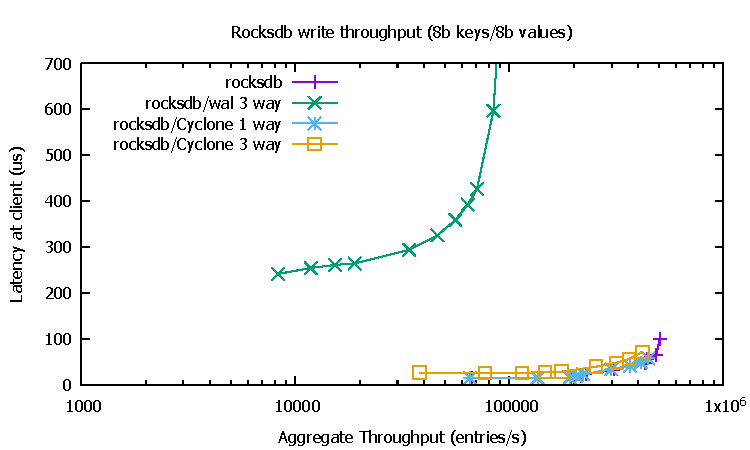
\includegraphics[scale=0.6]{results2/rocksdb.pdf}
\caption{Rocksdb - small updates}
\label{fig:rocksdb}
\end{figure}

\begin{figure}
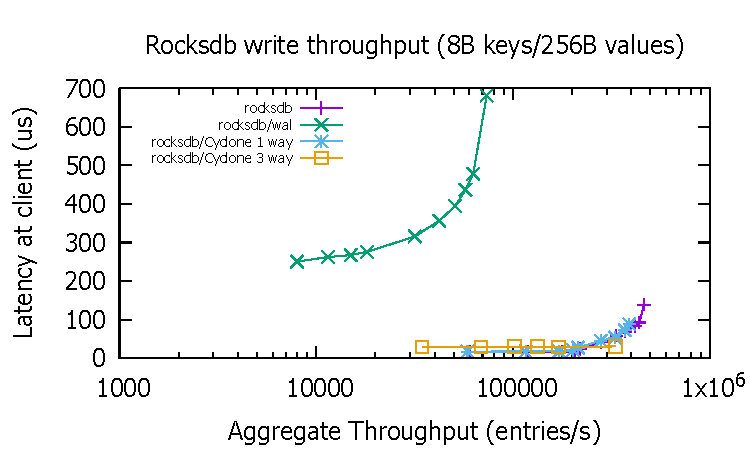
\includegraphics[scale=0.6]{results2/rocksdb_256.pdf}
\caption{Rocksdb - large updates}
\label{fig:rocksdb_256}
\end{figure}

Next, we consider the problem of supporting Rocksdb's write-batch operation that
atomically writes a set of key-value pairs into the KV store. In order to
perform the operation with Cyclone managing the log, the client must issue a
ganged operation across cores owning the keys in the write batch. This is in
contrast to baseline Rocksdb where the entire write batch can be sent to any
core. A key concern here was whether Cyclone would add any latency to the
operation due to the extra synchronization needed across replication quorums and
participating application cores. We examine the problem for the unloaded case
and small updates in Figure~\ref{fig:rocksdb_multi} for a single client with
increasing number of keys in the batch - till 32 keys that covers all
application cores. The line labeled Rocksdb is with no write-ahead logging. We
note an increasing latency for this baseline indicating Rocksdb takes longer
with larger key batches. For the other options - Rocksdb/wal has considerably
larger latency. Cyclone does an effective job of cutting down on this latency
even as it needs to pay a price for synchronizing multiple quorums and
application cores making it somewhat slower than running Rocksdb with no logging
for batched writes.

\begin{figure}
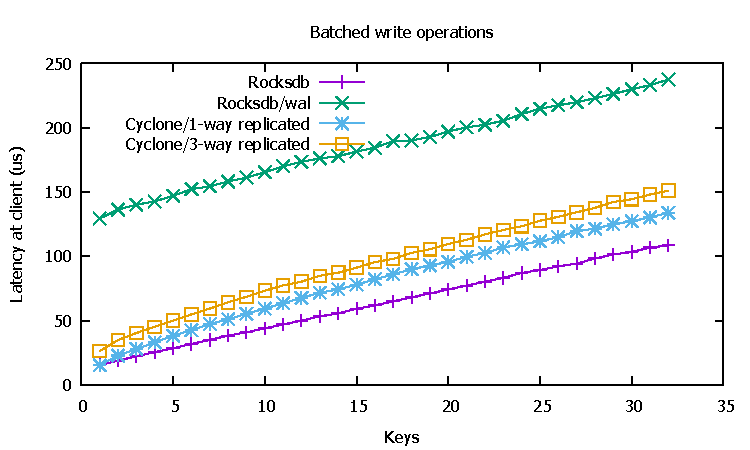
\includegraphics[scale=0.6]{results2/rocksdb_multi.pdf}
\caption{Rocksdb - batched writes}
\label{fig:rocksdb_multi}
\end{figure}

Finally we showcase the benefit of using Cyclone beyond pure performance as
compared to the existing single machine Rocksdb write ahead log. Cyclone brings
multi-machine availability with the ability to automatically failover. We
demonstrate this in Figure ~\ref{fig:timeline} that shows the timeline of a run
where we kill the server process on the leader replica. Cyclone is configured to
with a 30ms failure detection timeout after which the client library tries
replicas in turn to locate the leader - in this case it fails over in about
60ms.

\begin{figure}
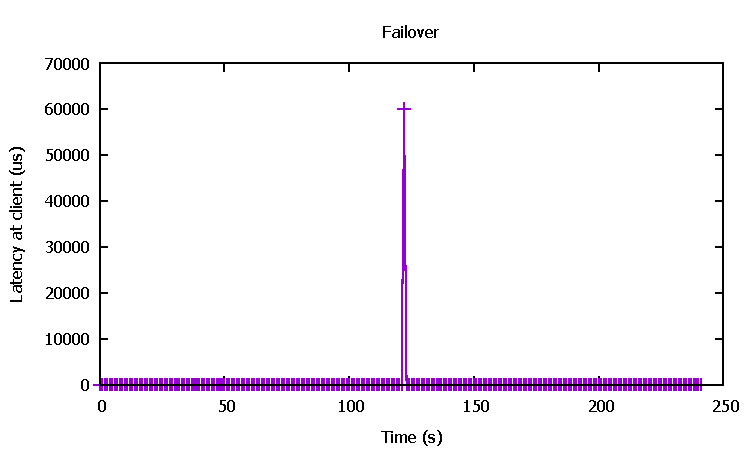
\includegraphics[scale=0.6]{results2/failover.pdf}
\caption{Rocksdb - failover}
\label{fig:timeline}
\end{figure}


\section{Related Work}
Memory technology in datacenters is due to undergo a paradigm shift with the
increased use of directly addressable non-volatile memory both in the form of
battery backed non-volatile DIMMs~\cite{farm} as well as newer memory types such
as 3D XPoint~\cite{pmfs, bpfs}. In anticipation, libraries that allow
programmers to build durable data structures on non-volatile heaps have become
available~\cite{mnemosyne, nvheaps, cdds} - an example of such a library that we
have used in this paper is Intel's non volatile memory library
(NVML)~\cite{nvml}. A missing piece however is a component to make such durable
data structures highly available using replication across a commodity network
such as ethernet. Existing solutions that offer good performance are dependent
on high performance RDMA networking hardware, with a dependence on external
services (such as zookeeper~\cite{zookeeper}) and application specific code for
fault recovery~\cite{farm, htm}.  This is a problem for programmers using NVML
where one cannot apriori guarantee the availability of such RDMA networking
hardware (for e.g., when running on externally hosted environments or public
clouds).

\section{Conclusion}
Cyclone allows developers to add availability to key value maps built on top of
libraries such as NVML and achieve good performance on commodity networking
hardware. A key question is whether Cyclone can be used for other applications
such as filesystems? \emph{We believe that the requirement for scaling across
  multiple replication quorums can be satisfied by applications where the
  scalable commutativity rule~\cite{scalable_commutativity} applies to common
  case primitives.} Although our intitial release of Cyclone will be for key
value style applications, our on-going research is based on the scalable
commutativity hypothesis.
\newcommand\myurl[2]{\url{#1}}
\bibliographystyle{plain}
\bibliography{paper}

\end{document}



